% !TEX root = ./article.tex

\documentclass{article}

\usepackage{mystyle}
\usepackage{myvars}

%-----------------------------

\begin{document}

	\maketitle
  \thispagestyle{empty}

%-----------------------------
%	TEXT
%-----------------------------

  \section{Transformación de la Función de Densidad}

    \paragraph{}
    Para realizar obtener la función de densidad de la transformación se utiliza la ecuación \eqref{eq:density_transformation_technique}, que relaciona una variable con su transformación. Se denomina $X$ a la variable aleatoria de origen, $Y = g(X)$ a la variable obtenida tras la transformación definida por la función $g$, cuya inversa es $g^{-1}$. Las funciones de densidad de $X$ e $Y$ se denominan $f_X$ y $f_Y$ respectivamente.

    \paragraph{}
    La ecuación \eqref{eq:density_transformation_technique} se define como una suma de funciones a trozos, particionadas de tal manera que cada tramo sea una función inyectiva. Nótese que (por la definición de función de densidad) la imagen de esta función deberá pertenecer al intervalor $[0,1]$, eliminando del soporte de $Y$ los casos en que esta restricción no se cumpla.

    \begin{equation}
    \label{eq:density_transformation_technique}
      f_Y (y) = \sum f_X \left( g^{-1} (y) \right) \left| \frac{d}{dy} g^{-1} (y) \right|
    \end{equation}

  \section{Ejercicios}

	\subsection{Sea $X$ una v. a. normal con media $\mu = 0$ y varianza $\sigma^2 = 1$, es decir, $ X \sim N(0,1)$. Hallar la función de densidad de la v.a. $Y = X^2$}

    \paragraph{}
    Para obtener la función de densidad de la variable transformada se seguirá la ecuación \eqref{eq:density_transformation_technique}, por lo tanto, lo primero es definir $f_X(x)$, $g(x)$, $g^{-1}(x)$ y $\left| \frac{d}{dx} g^{-1} (x) \right|$:

    \begin{align}
    \label{eq:e1_1}
      f_X(x) =& {\displaystyle {\frac {1}{\sqrt {2\pi \sigma ^{2}}}}\,e^{-{\frac {(x-\mu )^{2}}{2\sigma ^{2}}}}} = \frac{1}{\sqrt{2\pi} } e^{-\frac{x^2}{2}}, \ x \in \mathbb{R} \\
    \label{eq:e1_2}
      g(x) =& x^2 \\
    \label{eq:e1_3}
      g^{-1}(x) =& \pm \sqrt{x} \\
    \label{eq:e1_4}
      \left| \frac{d}{dx} g^{-1} (x) \right| =& \left| \pm \frac{1}{2\sqrt{x}}  \right| = \frac{1}{2\sqrt{x}}
    \end{align}

    \paragraph{}
    Tal y como se puede apreciar en la figura \ref{fig:x_square_plot}, $g(x)$ puede representarse a partir de dos funciones inyectivas, que además son simétricas entre sí. Lo cual es útil en el proceso de derivación de la función $f_Y$ siguiendo la ecuación \eqref{eq:density_transformation_technique}, la cual se realiza en las ecuaciónes \eqref{eq:e1_5} - \eqref{eq:e1_12}. En la ecuación \eqref{eq:e1_7} simplemente se sustituyen todas las variables por las indicadas anteriormente. En \eqref{eq:e1_8} se utiliza la propiedad de simetría.

    \paragraph{}
    El resto de cálculos se basan en simplifación hasta llegar a \eqref{eq:e1_12}, donde se ha indicado el soporte de la variable $Y$ (todos los reales positivos sin el cero). Se podría haber llegado a esta conclusión estudiando las función $g$ puesto que su imagen es  $\mathbb{R^*}$. En la figura \ref{fig:e1_f_x_f_y} se puede visualizar de manera gráfica la relación entre $f_X$ y $f_Y$.

    \begin{figure}
      \centering
      \begin{minipage}[b]{0.4\textwidth}
        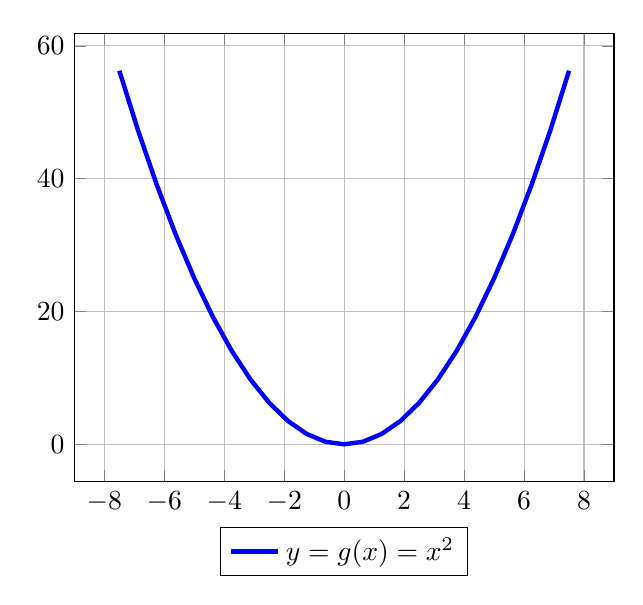
\begin{tikzpicture}
            \begin{axis}[
              legend style={
                at={(0.5,-0.1)},
                anchor=north,
                legend columns=-1
              },
              grid=both,
              xtick distance=2,
              every axis plot/.append style={ultra thick}
            ]
              \addplot[color=blue][domain=-7.5:7.5]{x^2};
            \legend{$y = g(x) = x^2$}
            \end{axis}
        \end{tikzpicture}
        \caption{}
        \label{fig:x_square_plot}
      \end{minipage}
      \hfill
      \begin{minipage}[b]{0.4\textwidth}
        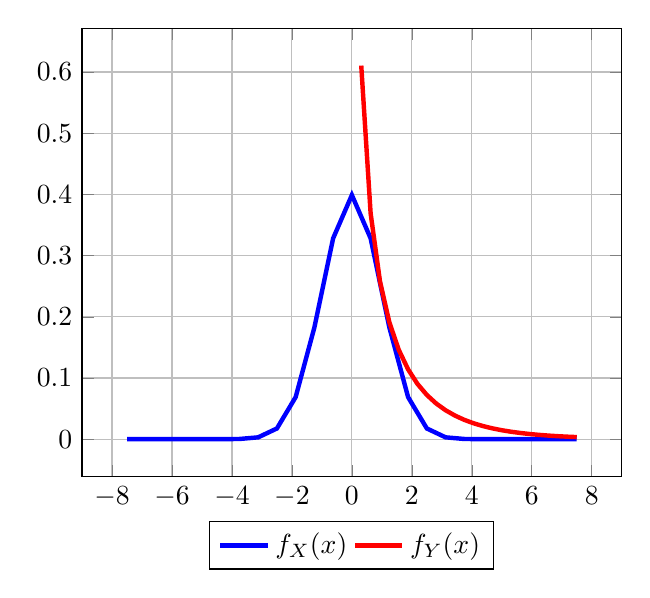
\begin{tikzpicture}
            \begin{axis}[
              legend style={
                at={(0.5,-0.1)},
                anchor=north,
                legend columns=-1
              },
              grid=both,
              xtick distance=2,
              ytick distance=0.1,
              every axis plot/.append style={ultra thick}
            ]
              \addplot[color=blue][domain=-7.5:7.5]{e^(- (x^2 / 2))/(sqrt(2 * pi))};
              \addplot[color=red][domain=0:7.5] {e^(-x / 2)/(sqrt(2 * pi)*sqrt(x))};
            \legend{ $f_X(x)$, $f_Y(x)$}
            \end{axis}
        \end{tikzpicture}
        \caption{}
        \label{fig:e1_f_x_f_y}
      \end{minipage}
    \end{figure}


    \begin{align}
    \label{eq:e1_5}
      f_Y (y) =& &\\
    \label{eq:e1_6}
              =& \sum f_X \left( g^{-1} (y) \right) \left| \frac{d}{dy} g^{-1} (y) \right| &\\
    \label{eq:e1_7}
              =& f_X \left( \sqrt{y} \right) \left| \frac{d}{dy} g^{-1} (y) \right| + f_X \left( - \sqrt{y} \right) \left| \frac{d}{dy} g^{-1} (y) \right| &\\
    \label{eq:e1_8}
              =& 2f_X \left( \sqrt{y} \right) \left| \frac{d}{dy} g^{-1} (y) \right| &\\
    \label{eq:e1_9}
              =& 2f_X \left( \sqrt{y} \right) \left| \pm \frac{1}{2\sqrt{y}} \right| &\\
    \label{eq:e1_10}
              =& 2f_X \left( \sqrt{y} \right) \frac{1}{2\sqrt{y}} &\\
    \label{eq:e1_11}
              =& 2\frac{1}{\sqrt{2\pi} } e^{-\frac{y}{2}} \frac{1}{2\sqrt{y}}  & \\
    \label{eq:e1_12}
              =& \frac{e^{-\frac{y}{2}}}{ \sqrt{2\pi} \sqrt{y} } & 0<y<\infty
    \end{align}

    \paragraph{}
    Debido a

  \subsection{Sea $X$ una v. a. uniformemente distribuida en $[0,2\pi]$, es decir, con función de densidad $f(x)=\frac{1}{2\pi}, \ x \in (0,2\pi)$. Hallar la función de densidad de la v.a. $Y = \cos(X)$}

    \paragraph{}
    Al igual que en el ejercicio anterior, para obtener la función de densidad de la variable transformada se seguirá la ecuación \eqref{eq:density_transformation_technique}, por lo tanto, lo primero es definir $f_X(x)$, $g(x)$, $g^{-1}(x)$ y $\left| \frac{d}{dx} g^{-1} (x) \right|$:

    \begin{align}
    \label{eq:e2_1}
      f_X(x) =& \frac{1}{2\pi}, \ 0 < x < 2\pi \\
    \label{eq:e2_2}
      g(x) =& \cos(x) \\
    \label{eq:e2_3}
      g^{-1}(x) =& \arccos(x) \\
    \label{eq:e2_4}
      \left| \frac{d}{dx} g^{-1} (x) \right| =& \left| - \frac{1}{\sqrt{1-x^2}} \right| =  \frac{1}{\sqrt{1-x^2}}
    \end{align}

    \begin{figure}
      \centering
      \begin{minipage}[b]{0.4\textwidth}
        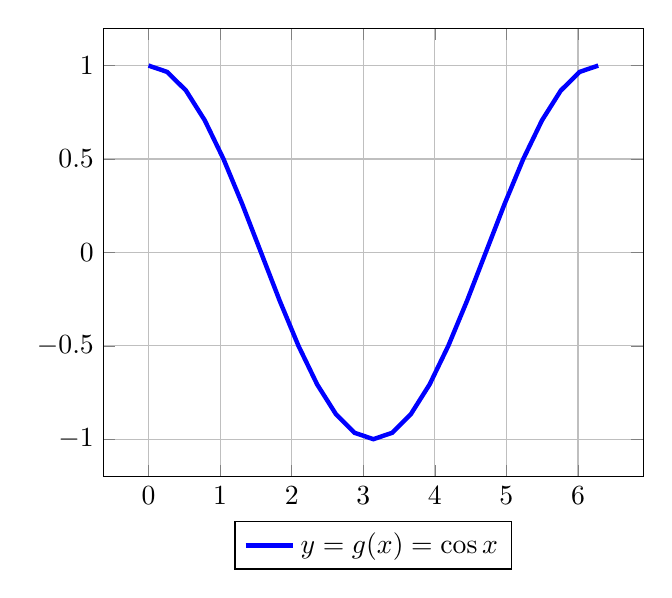
\begin{tikzpicture}
            \begin{axis}[
              legend style={
                at={(0.5,-0.1)},
                anchor=north,
                legend columns=-1
              },
              grid=both,
              xtick distance=1,
              ytick distance=0.5,
              every axis plot/.append style={ultra thick}
            ]
              \addplot[color=blue][domain=0:2*pi]{cos(deg(x))};
            \legend{$y = g(x) = \cos{x}$}
            \end{axis}
        \end{tikzpicture}
        \caption{}
        \label{fig:cos_x_plot}
      \end{minipage}
      \hfill
      \begin{minipage}[b]{0.4\textwidth}
        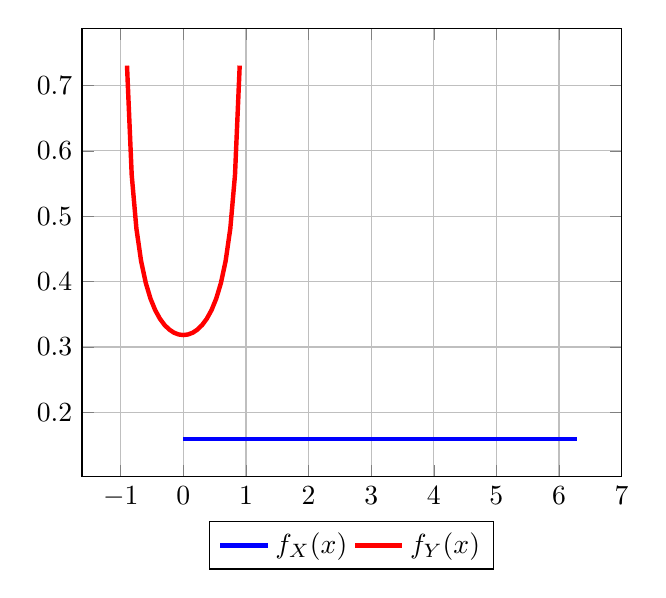
\begin{tikzpicture}
            \begin{axis}[
              legend style={
                at={(0.5,-0.1)},
                anchor=north,
                legend columns=-1
              },
              grid=both,
              xtick distance=1,
              ytick distance=0.1,
              every axis plot/.append style={ultra thick}
            ]
              \addplot[color=blue][domain=0:2*pi]{1/(2*pi)};
              \addplot[color=red][domain=-0.9:0.9] {1 / (pi * sqrt(1-x^2))};
            \legend{ $f_X(x)$, $f_Y(x)$}
            \end{axis}
        \end{tikzpicture}
        \caption{}
        \label{fig:e2_f_x_f_y}
      \end{minipage}
    \end{figure}

    \begin{align}
    \label{eq:e2_5}
      f_Y (y) =& &\\
    \label{eq:e2_6}
              =& \sum f_X \left( g^{-1} (y) \right) \left| \frac{d}{dy} g^{-1} (y) \right| &\\
    \label{eq:e2_7}
              =& 2\frac{1}{2\pi} \left| \frac{d}{dy} g^{-1} (y) \right| &\\
    \label{eq:e2_8}
              =& 2\frac{1}{2\pi}*\frac{1}{\sqrt{1-y^2}} &\\
    \label{eq:e2_9}
              =& \frac{1}{\pi\sqrt{1-y^2}} & -1<y<1
    \end{align}
%-----------------------------
%	Bibliographic references
%-----------------------------
  \nocite{prob2017}

  \bibliographystyle{alpha}
  \bibliography{bib}

\end{document}
